\chapter{Algoritmo de Detección de Sismos}

Uno de los objetivos específicos de esta tesis es proveer una metodología para detectar la ocurrencia de sismos. Con la finalidad de mejorar el trabajo realizado en estado del arte, se busca que la metodología propuesta no dependa de procesos de clasificación supervisada de los mensajes (por lo tanto, que no requiera costos asociados al trabajo de etiquetado), y que permita detectar sismos correctamente en tiempo cercano al \textit{tiempo real}, usando el flujo de mensajes publicados en Twitter. Además, el enfoque utilizado pretende detectar actividad sísmica en cualquier parte del mundo de una manera simple. 

El algoritmo propuesto es una adaptación de un enfoque existente de detección de anomalías en flujos de texto \jm{agregar ref}. Esta propuesta formaliza y generaliza el algoritmo presentado por \jm{agregar ref} para ser utilizado para monitorear señales discretas genéricas que son creadas agrupando datos relacionados con sismos extraídos desde el flujo de mensajes de Twitter. Además se agrega un método que permite arrojar automáticamente una alerta cuando se detecta una variación positiva en la señal.

\jm{Explicación en detalle del trabajo de Jheser(?)}\jm{Basta con hacer la referencia(?) o además debo explicar que esto lo hizo principalmente Jheser(?)}

\section{Monitoreo de la Velocidad de Llegada Relativa}

La detección de anomalías propuesto por Guzman y Poblete~\cite{guzman2013line} está basada en cambios en la velocidad de llegada relativa ($\lambda$) de los mensajes que contienen ciertas palabras clave (mensajes relevantes).
%El método propuesto por Guzman y Poblete~\cite{guzman2013line} detecta cambios en la \textit{velocidad relativa de llegada} de los mensajes relevantes.

Para definir esto formalmente se considera ${\mathcal F} = \langle F_1, F_2, \dots, F_n \rangle$ un flujo de mensajes indexados por tiempo , donde  $t: {\mathcal F} \rightarrow \mathbb{R}^+$ indica el tiempo de llegada de los mensajes, $F_i \subseteq A$ es el conjunto de atributos del mensaje $F_i$ y $A$ es el conjunto de posibles atributos de los mensajes entre los que se encuentran las palabras clave, localidades, \textit{hashtags}, sentimiento inferido, entre otros.  

En el conjunto de posibles atributos en $A$ existen algunos que constituyen \emph{elementos de interés}, los cuales dependen de lo que se quiera detectar (en este caso, atributos que podrían estar relacionados con sismos) y que se denotan como $K \subseteq A$.

Además se denotan:
\begin{itemize}
	\item $w_i = \langle w^s_i, w^e_i \rangle$ como una ventana de tiempo que abarca desde el tiempo $w^s_i$ hasta el tiempo $w^e_i$.
 	\item $M_i = \{ s \in {\mathcal F}: w^s_i \le t(s) \le w^e_i \}$ como el conjunto de los mensajes de ${\mathcal F}$ dentro de la ventana de tiempo. 
	\item $\operatorname{freq}(K, M_i) = | \{ F \in M_i: K \cap F \neq \emptyset \} |$ como cantidad de mensajes dentro $M_i$ que contienen elementos de interés.
\end{itemize}

Finalmente, en el método propuesto, el flujo de datos es procesado en grupos, dividiendo los mensajes que llegan en ventanas de tiempo consecutivas de largo fijo $T$.

Considerando todo lo anterior, para una ventana de tiempo dada $w_i$ que contiene los mensajes $M_i$, se define la \emph{velocidad de llegada relativa} ($\lambda$) de elementos de interés en esta ventana como:

\begin{equation}
\label{eq:lambda}
\lambda(K, M_i) = \frac{\mathrm{freq}(K,M_i)}{T|M_i|}
\end{equation}


%La detección de anomalías propuesto por Guzman y Poblete~\cite{guzman2013line} está basada en cambios en la velocidad de llegada relativa ($\lambda$) de los mensajes que contienen ciertas palabras clave.
%
La metodología propuesta por Guzman y Poblete~\cite{guzman2013line} analiza el flujo de datos extraído de Twitter y a partir de él es capaz de detectar anomalías asociadas a ciertas palabras clave. 
%
En este trabajo de tesis, esa idea se formaliza y se extiende para ser aplicada sobre una entrada menos genérica de señales discretas (${\mathcal F}$) que se pueden generar a partir de un flujo de datos. 
%
La metodología aquí propuesta monitorea la señal en el tiempo, para determinar cuándo una variación positiva en la velocidad de llegada relativa ($\lambda$) en la señal es significativamente más grande que otras variaciones producidas por el ruido observado en el pasado.
%
Originalmente, en el método propuesto por Guzman y Poblete en~\cite{guzman2013line}, la ``explosividad'' de cada palabra es estimada en base a la magnitud del cambio de su velocidad de llegada relativa ($\lambda$) con respecto a la ventana de tiempo previa.
%
La salida es una lista de los top-\emph{k} términos ordenados en orden decreciente según el cambio de su velocidad de llegada relativa ($\lambda$).
%
Esto no es suficiente para el propósito de la detección de sismos, ya que se requiere monitorear pocas señales (menos que \emph{k} señales), las cuales experimentan pequeños cambios en cada ventana de tiempo debido a fluctuaciones al azar en los datos de entrada (i.e., ruido).
%
Por lo tanto, si se reportan las top-\emph{k} señales más ``explosivas'' podría significar tener reportes en cada ventana de tiempo.
%
Es por esto, que para reportar sismos automáticamente se necesita estimar, de forma confiable, cuándo un cambio es significante y por tanto indica actividad inusual.

\begin{figure}[ht]
\centering
	\begin{subfigure}{.5\textwidth}
		\centering
		\caption{Distribución de la frecuencia de los mensajes relacionados con sismos.} 
		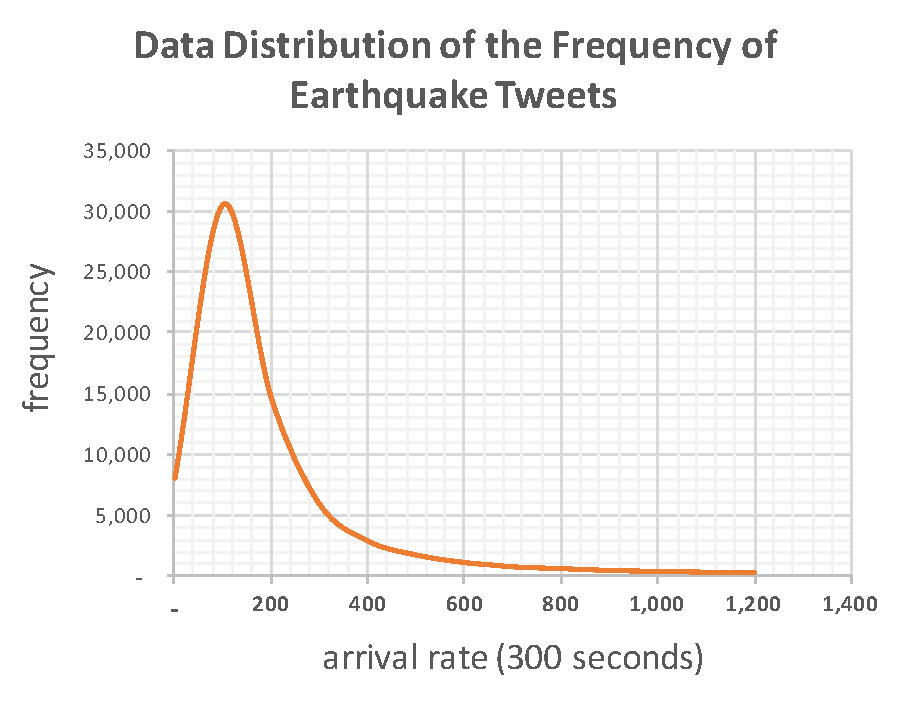
\includegraphics[trim={10 12 5 60}, clip, height=150pt]{imagenes/05_Data_Distribution1.pdf}
		\label{fig:data_distribution1}
		%\bp{Jheser: cambiar label-x por ``arrival rate (seconds)'' y label-y en minusculas}
  		%\jg{Resuelto: hice el cambio del label a 300 segundos ya que cada punto representa la ventana de 5mins. Si pongo solo segundos la escala del eje-x cambiaria en ambas figuras.}
  	\end{subfigure}% <- No quitar este comentario  	
  	\begin{subfigure}{.5\textwidth}
  		\centering
  		\caption{Distribución del logaritmo de la frecuencia de los mensajes relacionados con sismos.}
  		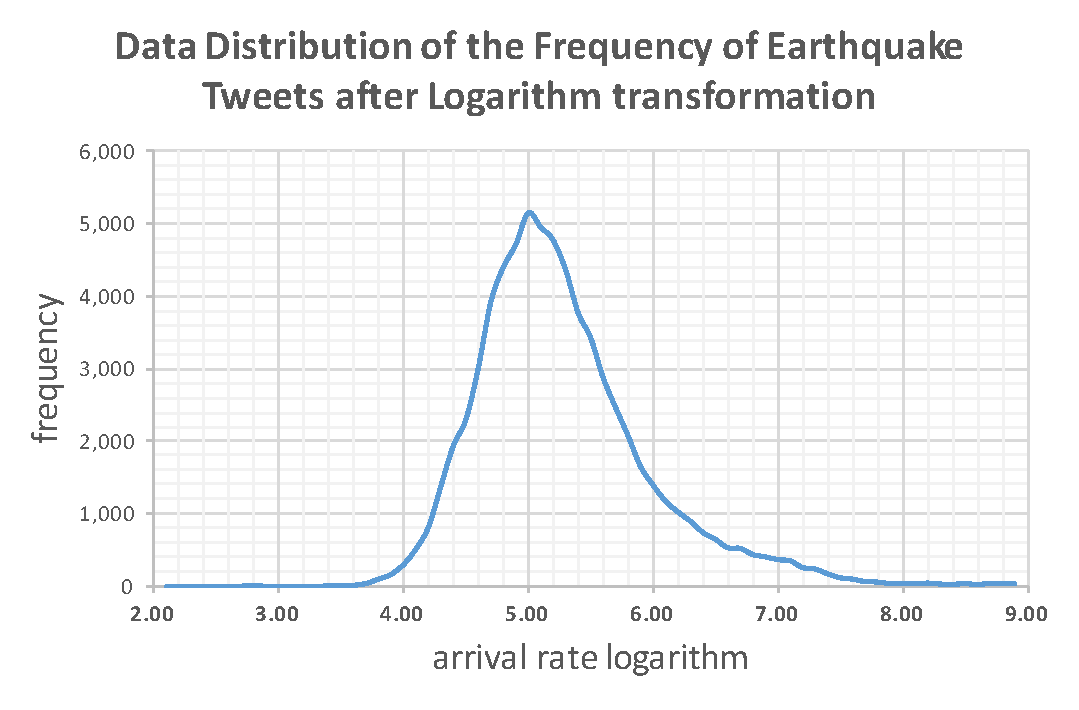
\includegraphics[trim={10 12 5 60}, clip,  height=150pt]{imagenes/05_Data_Distribution2.pdf}
  		\label{fig:data_distribution2}
  	\end{subfigure}
  	\caption{Distribución original de la frecuencia de mensajes relacionados con sismos y la distribución luego de aplicar la transformación logarítmica.}
\end{figure}


El enfoque natural para determinar si la velocidad relativa de llegada ($\lambda$) experimenta una variación significativa durante una ventana de tiempo $w_i$ es monitorear la desviación estándar de $\lambda$ para todas las ventanas de tiempo hasta $w_{i-1}$; al igual que como se ha hecho en el trabajo previo sobre detección de eventos emergentes usando enfoques estadísticos basados en la distribución de frecuencias~\cite{kleinberg2003bursty, mathioudakis2010twittermonitor,
nguyen2013event}.
%
Esta idea asume y requiere que la velocidad de llegada relativa ($\lambda$) tenga una distribución exponencial. 
%
Sin embargo, un análisis empírico cuyo resultado se muestra en la figura ~\ref{fig:data_distribution1}, usando el conjunto de datos descrito en la sección ~\ref{sec:dataset}, indica que esto no se cumple para el caso de la distribución de la velocidad de llegada de las palabras relacionadas con sismos.
%
Esta observación hizo necesario un análisis para identificar como adaptar el algoritmo a los propósitos descritos en esta tesis.

Entre los análisis realizados hay uno que particularmente fue útil para continuar. Se aplicó una transformación logarítmica a los datos, tal como se muestra en la figura~\ref{fig:data_distribution2}, después de lo cual los datos se asemejan a una distribución log-normal.
 
We apply a log transformation to the data, shown in
Figure~\ref{fig:data_distribution2}, after which the data resembles a
log-normal distribution. 
%
% 
%Section~\ref{sec:setup} provides evidence that earthquake-related keywords follow a {\em log-normal}
%arrival rate distribution, shown in Figures~\ref{fig:data_distribution1} and \ref{fig:data_distribution2}.
%
Therefore, instead of tracking changes in the relative arrival rate
($\lambda$), we model the distribution as if it were a log-normal and track the {\em logarithm of this function},
defined as $\tilde{\lambda}$:

\begin{equation}
\label{eq:log_lambda}
\tilde{\lambda}(K, M_i) = \frac{\ln\left(\mathrm{freq}(K,M_i)\right)}{t |M_i|}
\end{equation}

Using the transformed function $\tilde{\lambda}(K, M_i)$ we compute its {\em z}-score to track variations in the input signal's relative arrival rate.  We compute the {\em z}-score at time-window $w_i$ as

\newcommand{\zscore}{\ensuremath{z\textnormal{-}\mathrm{score}}}
\begin{equation}
\label{eq:zscore}
\zscore(K, M_i) = \frac{\tilde{\lambda}(K, M_i)-\mu_i}{\sigma_i}
\end{equation}

\noindent where $\mu_i$ and $\sigma_i$ are, respectively, the mean and standard deviation of the observed values of $\tilde\lambda$ during time windows $w_1, w_2, \dots, w_{i-1}$.

The proposed method triggers an alert warning that an earthquake has been detected when $\zscore(K, M_i) \ge \theta$, where $\theta$ is
an experimentally defined threshold.
%
Our experiments suggest setting $\theta=1.5$ as a value that gives good results in practice, as detailed in Section~\ref{sec:experimental}.
%
Additionally, as an a heuristic that gives good results in practice, we exclude from the computation of $\mu_i$ and $\sigma_i$ in Equation~\ref{eq:zscore} the time-windows for which alerts are triggered, hence the average rate corresponds to the average of ``non-earthquake'' time-windows.


\section{Metodología de Ajuste de Parámetros Óptimos}